\documentclass[12pt]{article}
\usepackage[utf8]{inputenc}
\usepackage[spanish]{babel}

%Fuente (compilarlo en Latex.pdf normal porque va más rápido y luego
%y al final insertarlo en Arial) DA ERROR
%\usepackage{fontspec}
%\setmainfont{Arial}

%Estructura de la Página
\usepackage[left=2.54cm,right=2.54cm,top=2.54cm,bottom=2.54cm]{geometry}

%Tablas
\usepackage{xcolor, colortbl}
\usepackage{array, multirow, multicol}
\usepackage[]{float}
\usepackage{pdflscape}

%Páginas en horizontal


%Pies de página y encabezado
\usepackage{fancyhdr}

%Comentario párrafos
\usepackage{verbatim}

%Paquete arquitectura página
\pagestyle{fancy}
\fancyhf{}
\lhead{Revisión Informe Ensayos Lote 2}
\rhead{CAF}
\rfoot{\thepage}
\lfoot{}

%Interlineado
\renewcommand{\baselinestretch}{0.5}



%Paquete Matemático
\usepackage{amsmath}
\usepackage{amsfonts}
\usepackage{amssymb}
\usepackage{breqn}

%Paquete para el código
% Paquetes Listing

\usepackage{listings}
\usepackage{xcolor}

%Settings 

\definecolor{codegreen}{rgb}{0,0.6,0}
\definecolor{codegray}{rgb}{0.5,0.5,0.5}
\definecolor{codepurple}{rgb}{0.58,0,0.82}
\definecolor{backcolour}{rgb}{0.95,0.95,0.92}


\lstdefinestyle{mystyle}{
 backgroundcolor=\color{backcolour},   
 commentstyle=\color{codegreen},
 keywordstyle=\color{magenta},
 numberstyle=\tiny\color{codegray},
 stringstyle=\color{codepurple},
 basicstyle=\ttfamily\footnotesize,
 breakatwhitespace=false,         
 breaklines=true,                 
 captionpos=b,                    
 keepspaces=true,                 
 numbers=left,                    
 numbersep=5pt,                  
 showspaces=false,                
 showstringspaces=false,
 showtabs=false,                  
 tabsize=2
}

\lstset{style=mystyle}
%Paquete Imágenes

\usepackage{graphicx}
\graphicspath{ {Images/} }
\usepackage{subfig}

%Bibliografía
\usepackage[backend=bibtex]{biblatex}
\addbibresource{referencias.bib}

%Espacio entre párrafos
\setlength{\parskip}{0.5cm}
%Sangría
\setlength{\parindent}{0cm}

\title{Estudio de los rendimentos declarados  obtenidos para el motor de TSA implementado en el proyecto C.J5}
\author{José Honrubia Blanco}
\date{Noviembre 2022}

\begin{document}
\section{Objetivo}
El objetivo de este documento es comparar los valores calculados del motor TSA usado en el proyecto C.J5 con los valores finalmente obtenidos

\section{Método de Cálculo}
Los cálculos se van a realizar para las frecuencias de 30, 62.2, 71, 75 y 95 Hz. Al final, se hará la comparativa entre los puntos recogidos en el datasheet y los obtenidos en los ensayos realizados por TSA.

Para la ilustración de los cálculos se va a emplear los datos de partida de 75 Hz por ser el punto característico del motor (S1). Los valores se recogen en la tabla \ref{table: valores_iniciales}:

{\extrarowheight
\renewcommand{\arraystretch}{2.25}
\begin{table}[H]
    \centering
    \begin{tabular}{cccccc}
    P1 (W) & P2 (W) & \eta  (\%) & s (\%) & M_{calculado} (Nm) & M_{medido} (Nm) \\ \hline
    6522   & 1026   & 15.7                     & 0.01   & 4.4             & 4            \\
    7556   & 2054   & 27.2                     & 0.02   & 8.7             & 8            \\
    8450   & 2946   & 34.9                     & 0.03   & 12.5            & 5.5          \\
    10001  & 4480   & 44.8                     & 0.04   & 19              & 13           \\
    12910  & 7373   & 57.1                     & 0.05   & 31.3            & 22.75        \\
    15333  & 9778   & 63.8                     & 0.05   & 41.5            & 32           \\
    22496  & 16875  & 75                       & 0.09   & 71.7            & 58.5         \\
    29499  & 23811  & 80.7                     & 0.12   & 101.1           & 96.5         \\
    36175  & 30405  & 84                       & 0.16   & 129.2           & 125.5        \\
    48821  & 42870  & 87.8                     & 0.22   & 182.2           & 176          \\
    74969  & 68520  & 91.4                     & 0.33   & 291.5           & 277.5        \\
    105908 & 98666  & 93.2                     & 0.48   & 420.4           & 421.25       \\
    127337 & 119382 & 93.8                     & 0.61   & 509.2           & 495          \\
    147162 & 138462 & 94.1                     & 0.72   & 591.1           & 594.5        \\
    168103 & 158594 & 94.3                     & 0.77   & 677.5           & 671.75       \\
    191525 & 180824 & 94.4                     & 0.93   & 773.6           & 762.75       \\
    212776 & 201008 & 94.5                     & 1.01   & 859.9           & 866.5        \\
    237633 & 224159 & 94.3                     & 1.21   & 962.7           & 958          \\
    266158 & 250876 & 94.3                     & 1.31   & 1078            & 1070.5       \\
    301400 & 283611 & 94.1                     & 1.45   & 1219.9          & 1202.5       \\ \hline
    \end{tabular}
    \caption{Valores aportados por TSA para la frecuencia de 75 Hz a distintas potencias}
    \label{tab: valores_iniciales}
    \end{table}}
Siendo:
\begin{itemize}
    \item \textbf{P1}: Potencia eléctrica de entrada
    \item \textbf{P2}: Potencia Mecánica calculada
    \item \textbf{$\eta$}: El rendimiento calculado
    \item \textbf{s}: el deslizamiento en tanto por ciento
    \item \textbf{$M_{calculado}$}: El momento calculado
    \item  \textbf{$M_{medido}$}: El momento medido
\end{itemize}

La potencia $P2$ se obtiene de multiplicar la velocidad angular por el momento calculado. Lo primero que se hace es calcular la velocidad angular con la siguiente ecuación:
\begin{equation}
{\omega = \frac{f \cdot 2 \phi }{N \cdot \left(1 - \frac{s}{100}\right)}}
\label{eqn:velocidad_angular}
\end{equation}

donde:
\begin{itemize}
    \item \textbf{$\omega$}: velocidad angular
    \item \textbf{f}: frecuencia en Herzios. Para este cáculo se emplean 75 Herzios
    \item \textbf{N}: número de polos del motor
    \item \textbf{s}: el deslizamiento
\end{itemize}
Por otro lado, la potencia mecánica medida se calcula como el producto de la velocidad angular por el momento medido y, por último, el rendimiento se calcula dividiendo la potencia mecánica medida por la potencia eléctrica. Se incluye la potencia mecánica calculada para comprobar que sea igual que la potencia $P2$. En la tabla \ref{tab:valores_finales} se recogen el resultado de los datos junto con los iniciales.


{\extrarowheight
\renewcommand{\arraystretch}{2.25}
    \begin{table}[H]
        \centering
        \begin{tabular}{cccccc}
P1 / W & P2 (W) & $\eta_{calc}$ (\%) & $Pot_{mec calc$ & $Pot_{mec obt}$ & $\eta_{obt}$ \\ \hline
6522   & 1026   & 15.7    & 1036.6                      & 942.4                      & 14.4                 \\
7556   & 2054   & 27.2    & 2049.5                      & 1884.6                     & 25.0                 \\
8450   & 2946   & 34.9    & 2944.4                      & 1295.5                     & 15.3                 \\
10001  & 4480   & 44.8    & 4475.0                      & 3061.8                     & 30.6                 \\
12910  & 7373   & 57.1    & 7371.2                      & 5357.7                     & 41.5                 \\
15333  & 9778   & 63.8    & 9773.3                      & 7536.1                     & 49.2                 \\
22496  & 16875  & 75      & 16878.7                     & 13771.3                    & 61.2                 \\
29499  & 23811  & 80.7    & 23792.5                     & 22710.0                    & 77.0                 \\
36175  & 30405  & 84      & 30393.3                     & 29522.9                    & 81.6                 \\
48821  & 42870  & 87.8    & 42835.4                     & 41377.8                    & 84.7                 \\
74969  & 68520  & 91.4    & 68456.4                     & 65168.6                    & 86.9                 \\
105908 & 98666  & 93.2    & 98579.0                     & 98778.3                    & 93.3                 \\
127337 & 119382 & 93.8    & 119245.6                    & 115920.2                   & 91.1                 \\
147162 & 138462 & 94.1    & 138271.9                    & 139067.2                   & 94.5                 \\
168103 & 158594 & 94.3    & 158403.0                    & 157058.6                   & 93.4                 \\
191525 & 180824 & 94.4    & 180580.0                    & 178047.4                   & 93.0                 \\
212776 & 201008 & 94.5    & 200562.8                    & 202102.2                   & 95.0                 \\
237633 & 224159 & 94.3    & 224086.2                    & 222992.2                   & 93.8                 \\
266158 & 250876 & 94.3    & 250670.4                    & 248926.4                   & 93.6                 \\
301400 & 283611 & 94.1    & 283264.4                    & 279224.1                   & 92.6                 \\ \hline
        \end{tabular}
        \caption{Valores aportados por TSA y calculados a 75 Hz y distintas potencias.}
        \label{tab:valores_finales}
        \end{table}
}


Se pude observar como las potencias $P2$ y la potencia calculada son similares y que los rendimientos calculados y medidos son distintos. Falta por comprobar si cumplen el 15 \% indicado por la norma. Para ello se hace el siguiente cálculo:
\begin{equation}
\xi = \frac{(100 - \eta_{obtenido})-(100-\eta_{calculado})}{100 - \eta{calculado}}\cdot 100 = \frac{\eta_{calculado}_\eta_{obtenido}}{100-\eta{calculado}}\cdot 100
\label{eqn:{error}}
\end{equation}
del que se obtienen los siguientes resultados:
{\extrarowheight
\renewcommand{\arraystretch}{2.25}
\begin{table}[H]
    \centering
    \begin{tabular}{cc}
P2 (W) & error (\%)                   \\ \hline
1026   & 1.5                          \\
2054   & 3.1                          \\
2946   & \cellcolor[HTML]{FD6864}30.0 \\
4480   & \cellcolor[HTML]{FD6864}25.7 \\
7373   & \cellcolor[HTML]{FD6864}36.4 \\
9778   & \cellcolor[HTML]{FD6864}40.4 \\
16875  & \cellcolor[HTML]{FD6864}55.2 \\
23811  & \cellcolor[HTML]{FE996B}19.3 \\
30405  & \cellcolor[HTML]{FE996B}15.2 \\
42870  & \cellcolor[HTML]{FD6864}25.1 \\
68520  & \cellcolor[HTML]{FD6864}52.0 \\
98666  & -1.6                         \\
119382 & \cellcolor[HTML]{FD6864}43.9 \\
138462 & -7.0                         \\
158594 & \cellcolor[HTML]{FE996B}16.0 \\
180824 & \cellcolor[HTML]{FD6864}25.9 \\
201008 & -9.4                         \\
224159 & 8.6                          \\
250876 & 12.9                         \\
283611 & \cellcolor[HTML]{FE996B}24.7 \\ \hline
    \end{tabular}
    \caption{Error rendimientos calculados y medidos}
    \label{tab:error}
    \end{table}
    }
Se han marcado en rojo aquellos valores que superan el 25\% de error y en naranja aquellas que superan el 15\%. Como se puede observar, se tienen:
\begin{itemize}
    \item Por encima del 25\% de error: 9
    \item Entre el 15\% y el 25\% de error: 4
    \item Por debajo del 15\% de error: 7
\end{itemize}

En el siguiente apartado se recogen las gráficas con los resultados de estos cálculos para las frecuencias mencionadas.

\section{Resultados}
\subsection{Frecuencia de 30 Hz}
\begin{figure}[H]
\centering
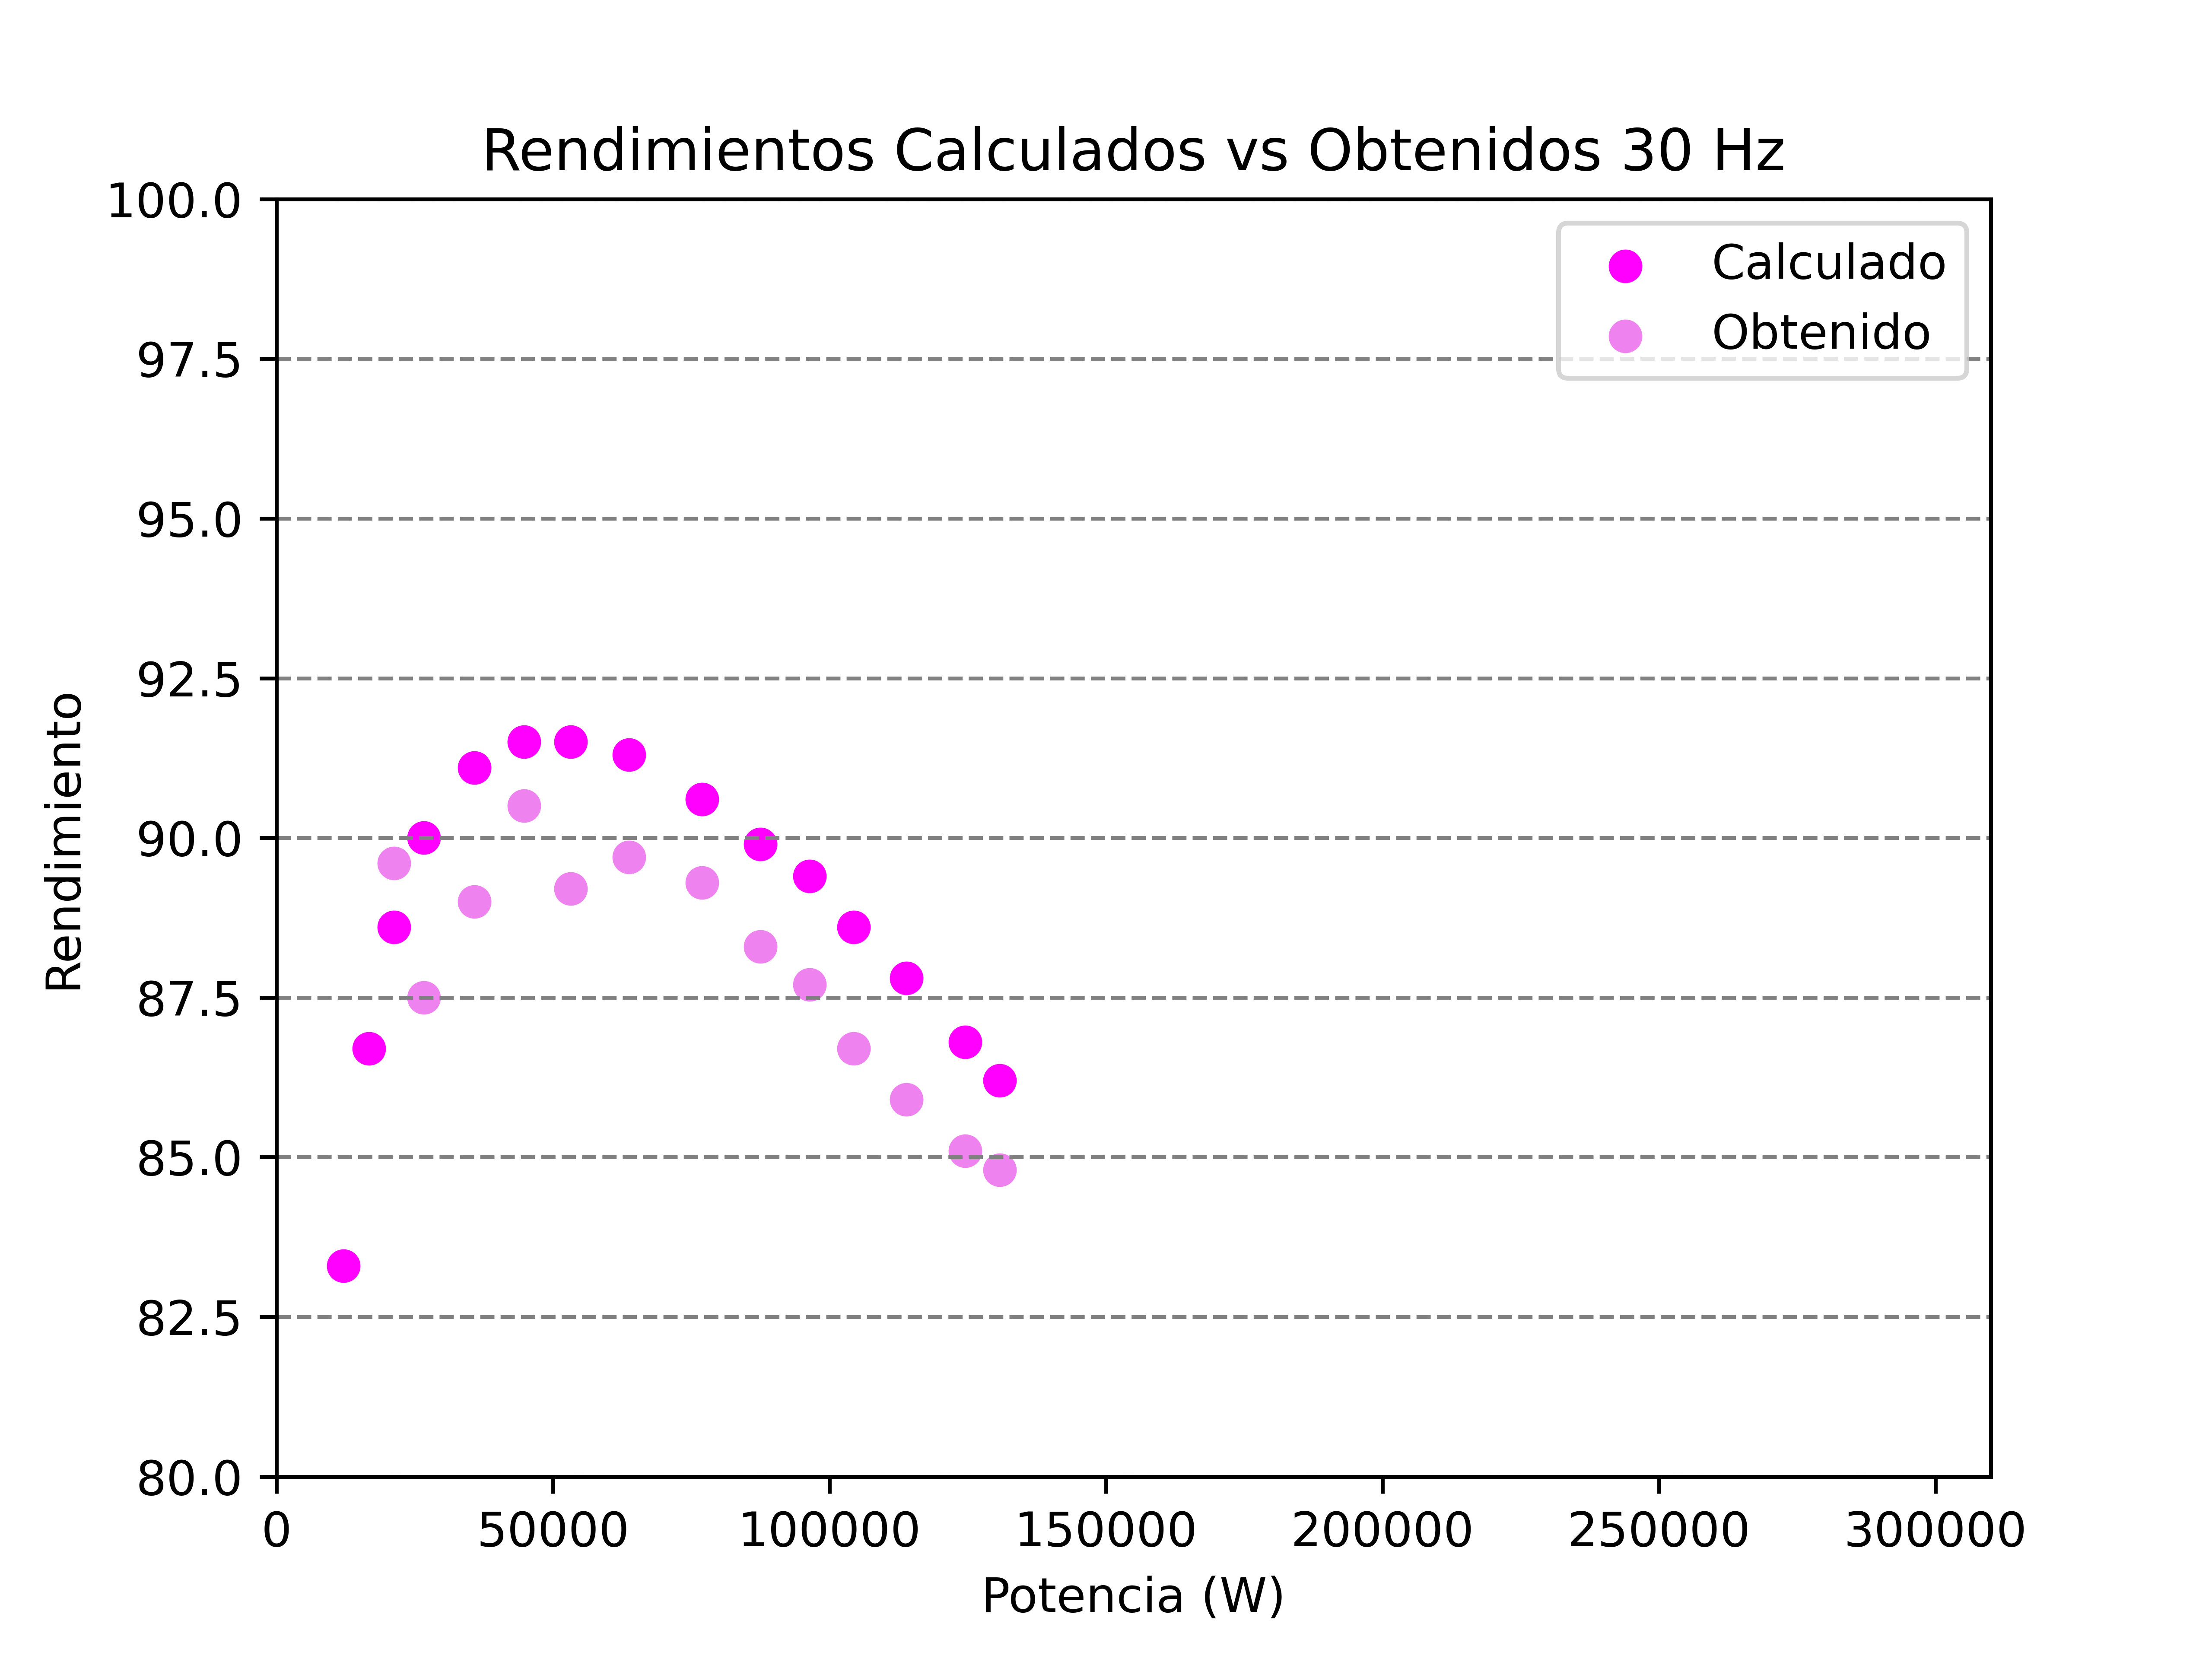
\includegraphics[width=0.6\textwidth]{Rendimientos Calculados vs Obtenidos 30 Hz.png}
\caption{}
\label{fig:}
\end{figure}

\begin{figure}[H]
\centering
\includegraphics[width=0.6\textwidth]{Desviacion Rendimientos (\%) 30 Hz.png}
\caption{}
\label{fig:}
\end{figure}

\subsection{Frecuencia de 62.2 Hz}
\begin{figure}[H]
\centering
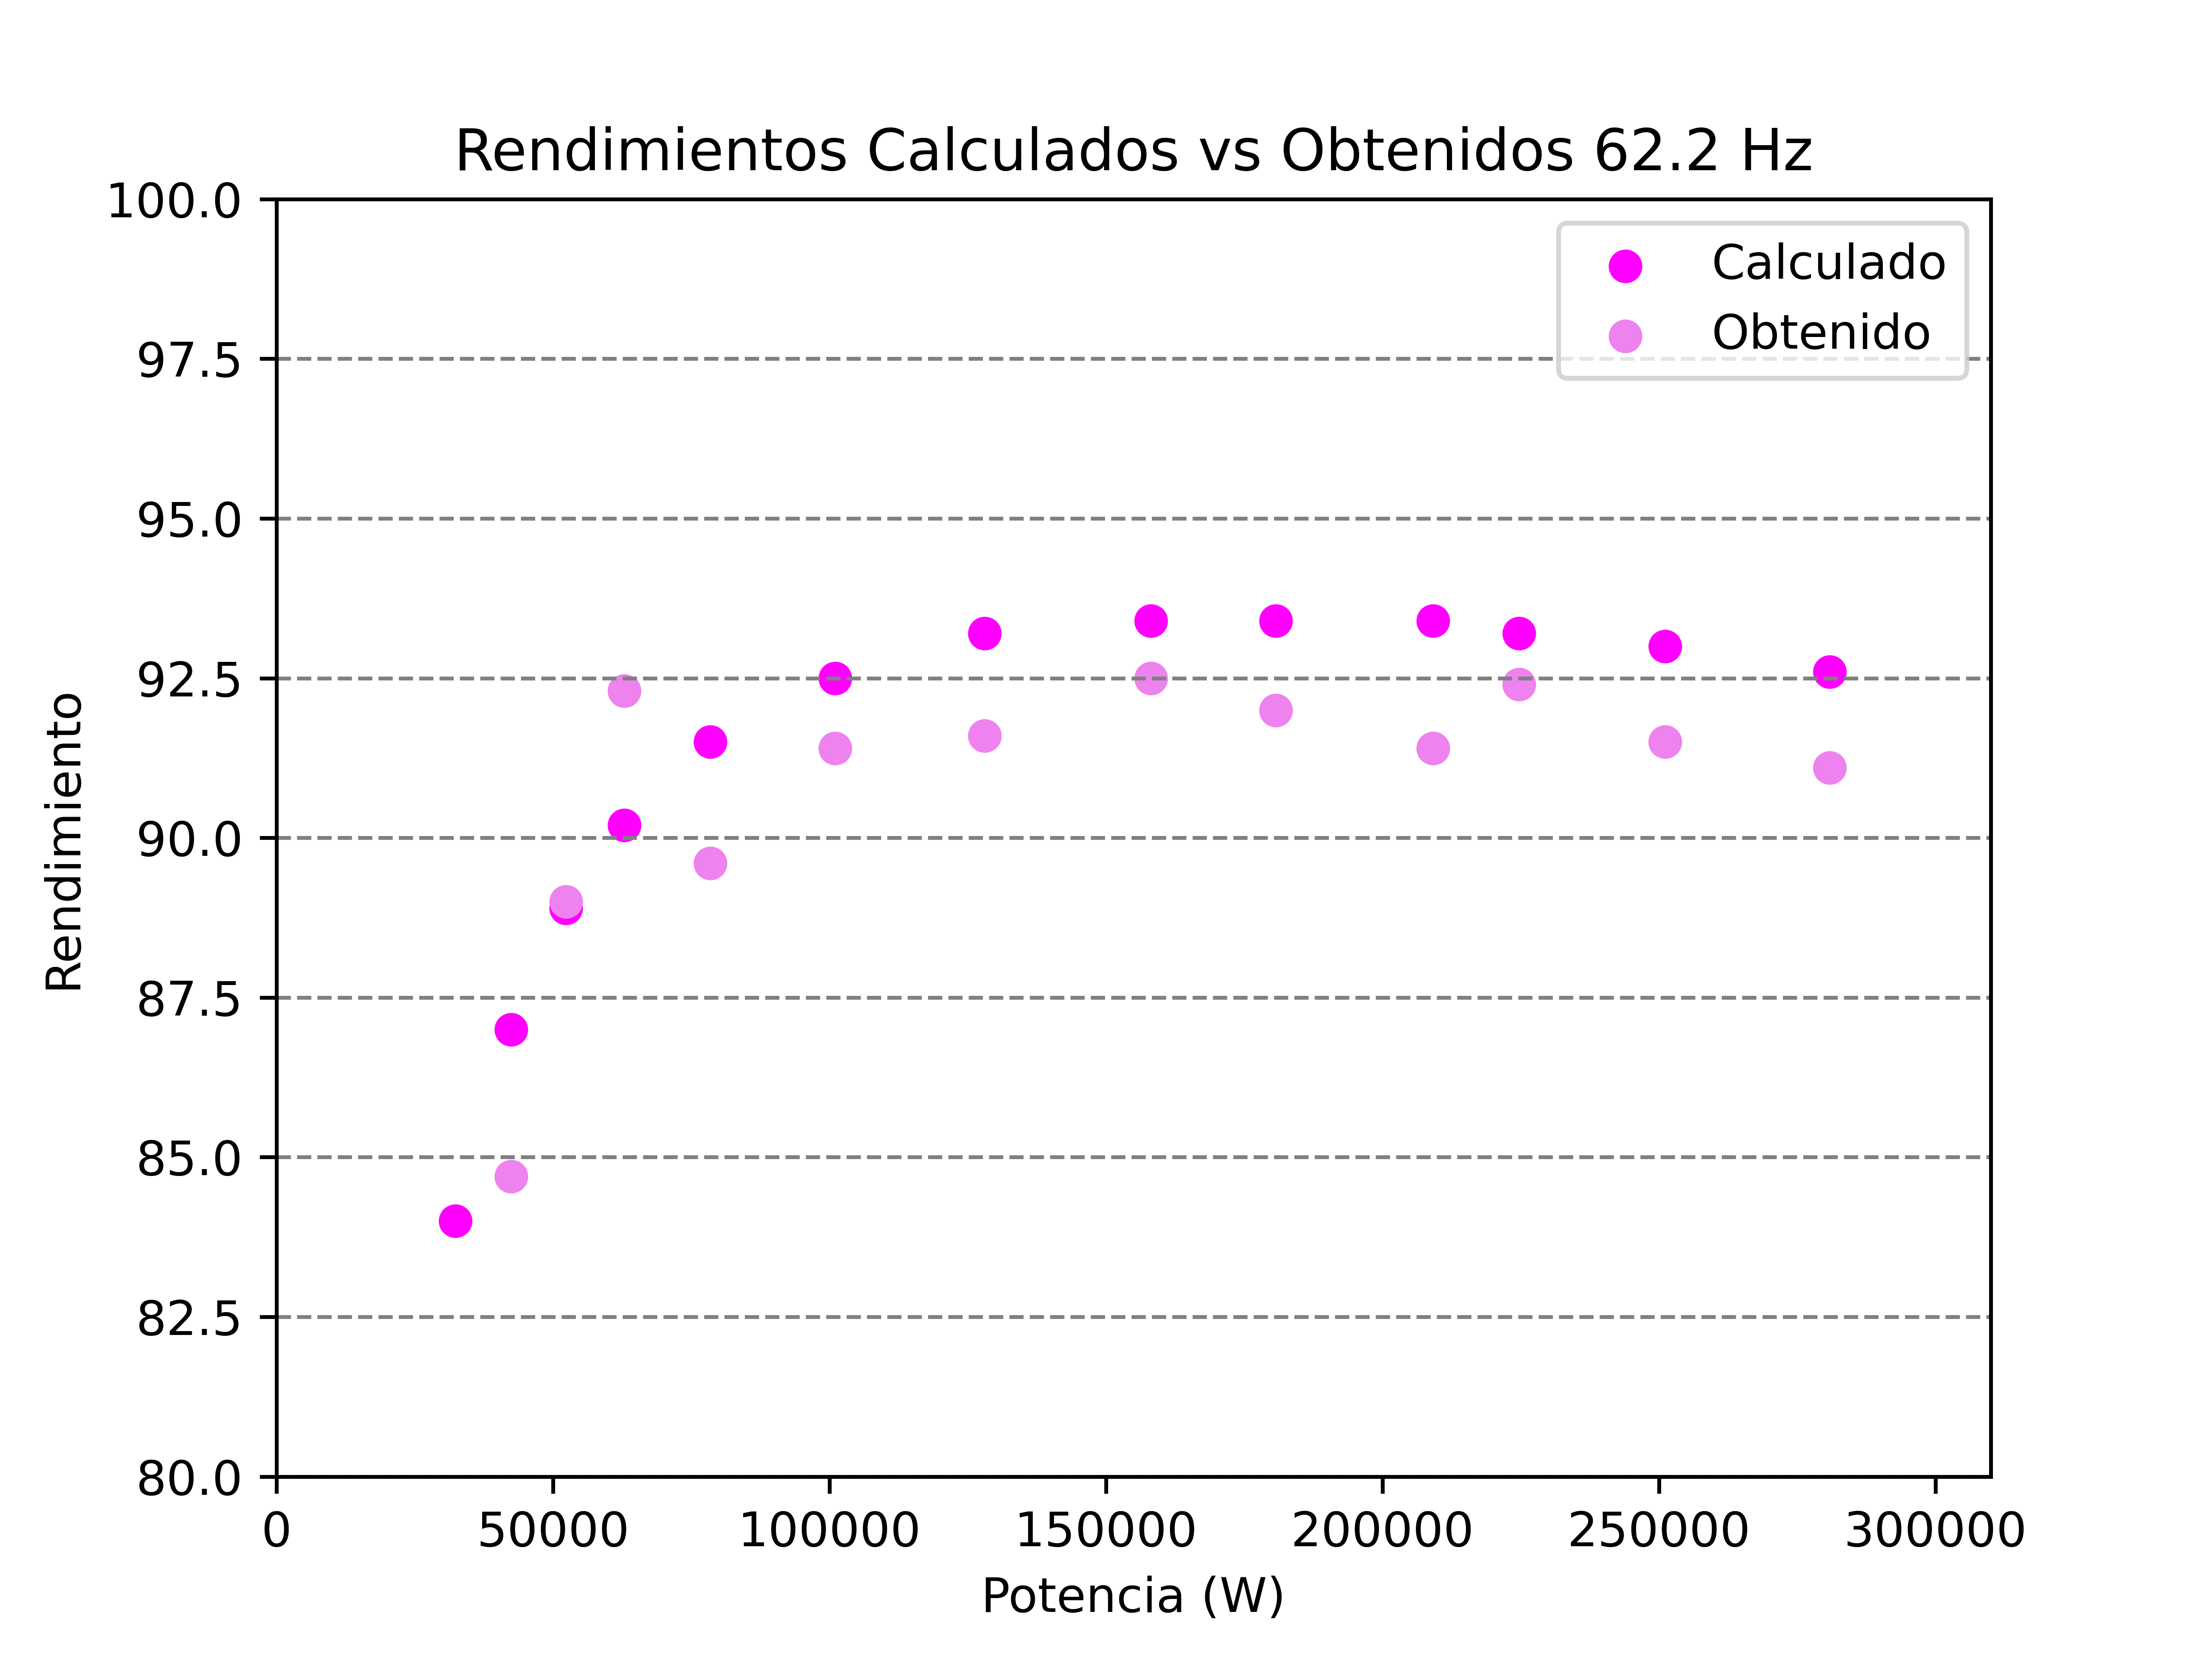
\includegraphics[ width=0.6\textwidth]{ Rendimientos Calculados vs Obtenidos 62.2 Hz.png }
\caption{}
\label{fig:}
\end{figure}
\begin{figure}[H]
\centering
\includegraphics[ width=0.6\textwidth]{ desviacion Rendimientos (\%) 62.2 Hz.png }
\caption{}
\label{fig:}
\end{figure}

\subsection{Frecuencia de 71 Hz}
\begin{figure}[H]
\centering
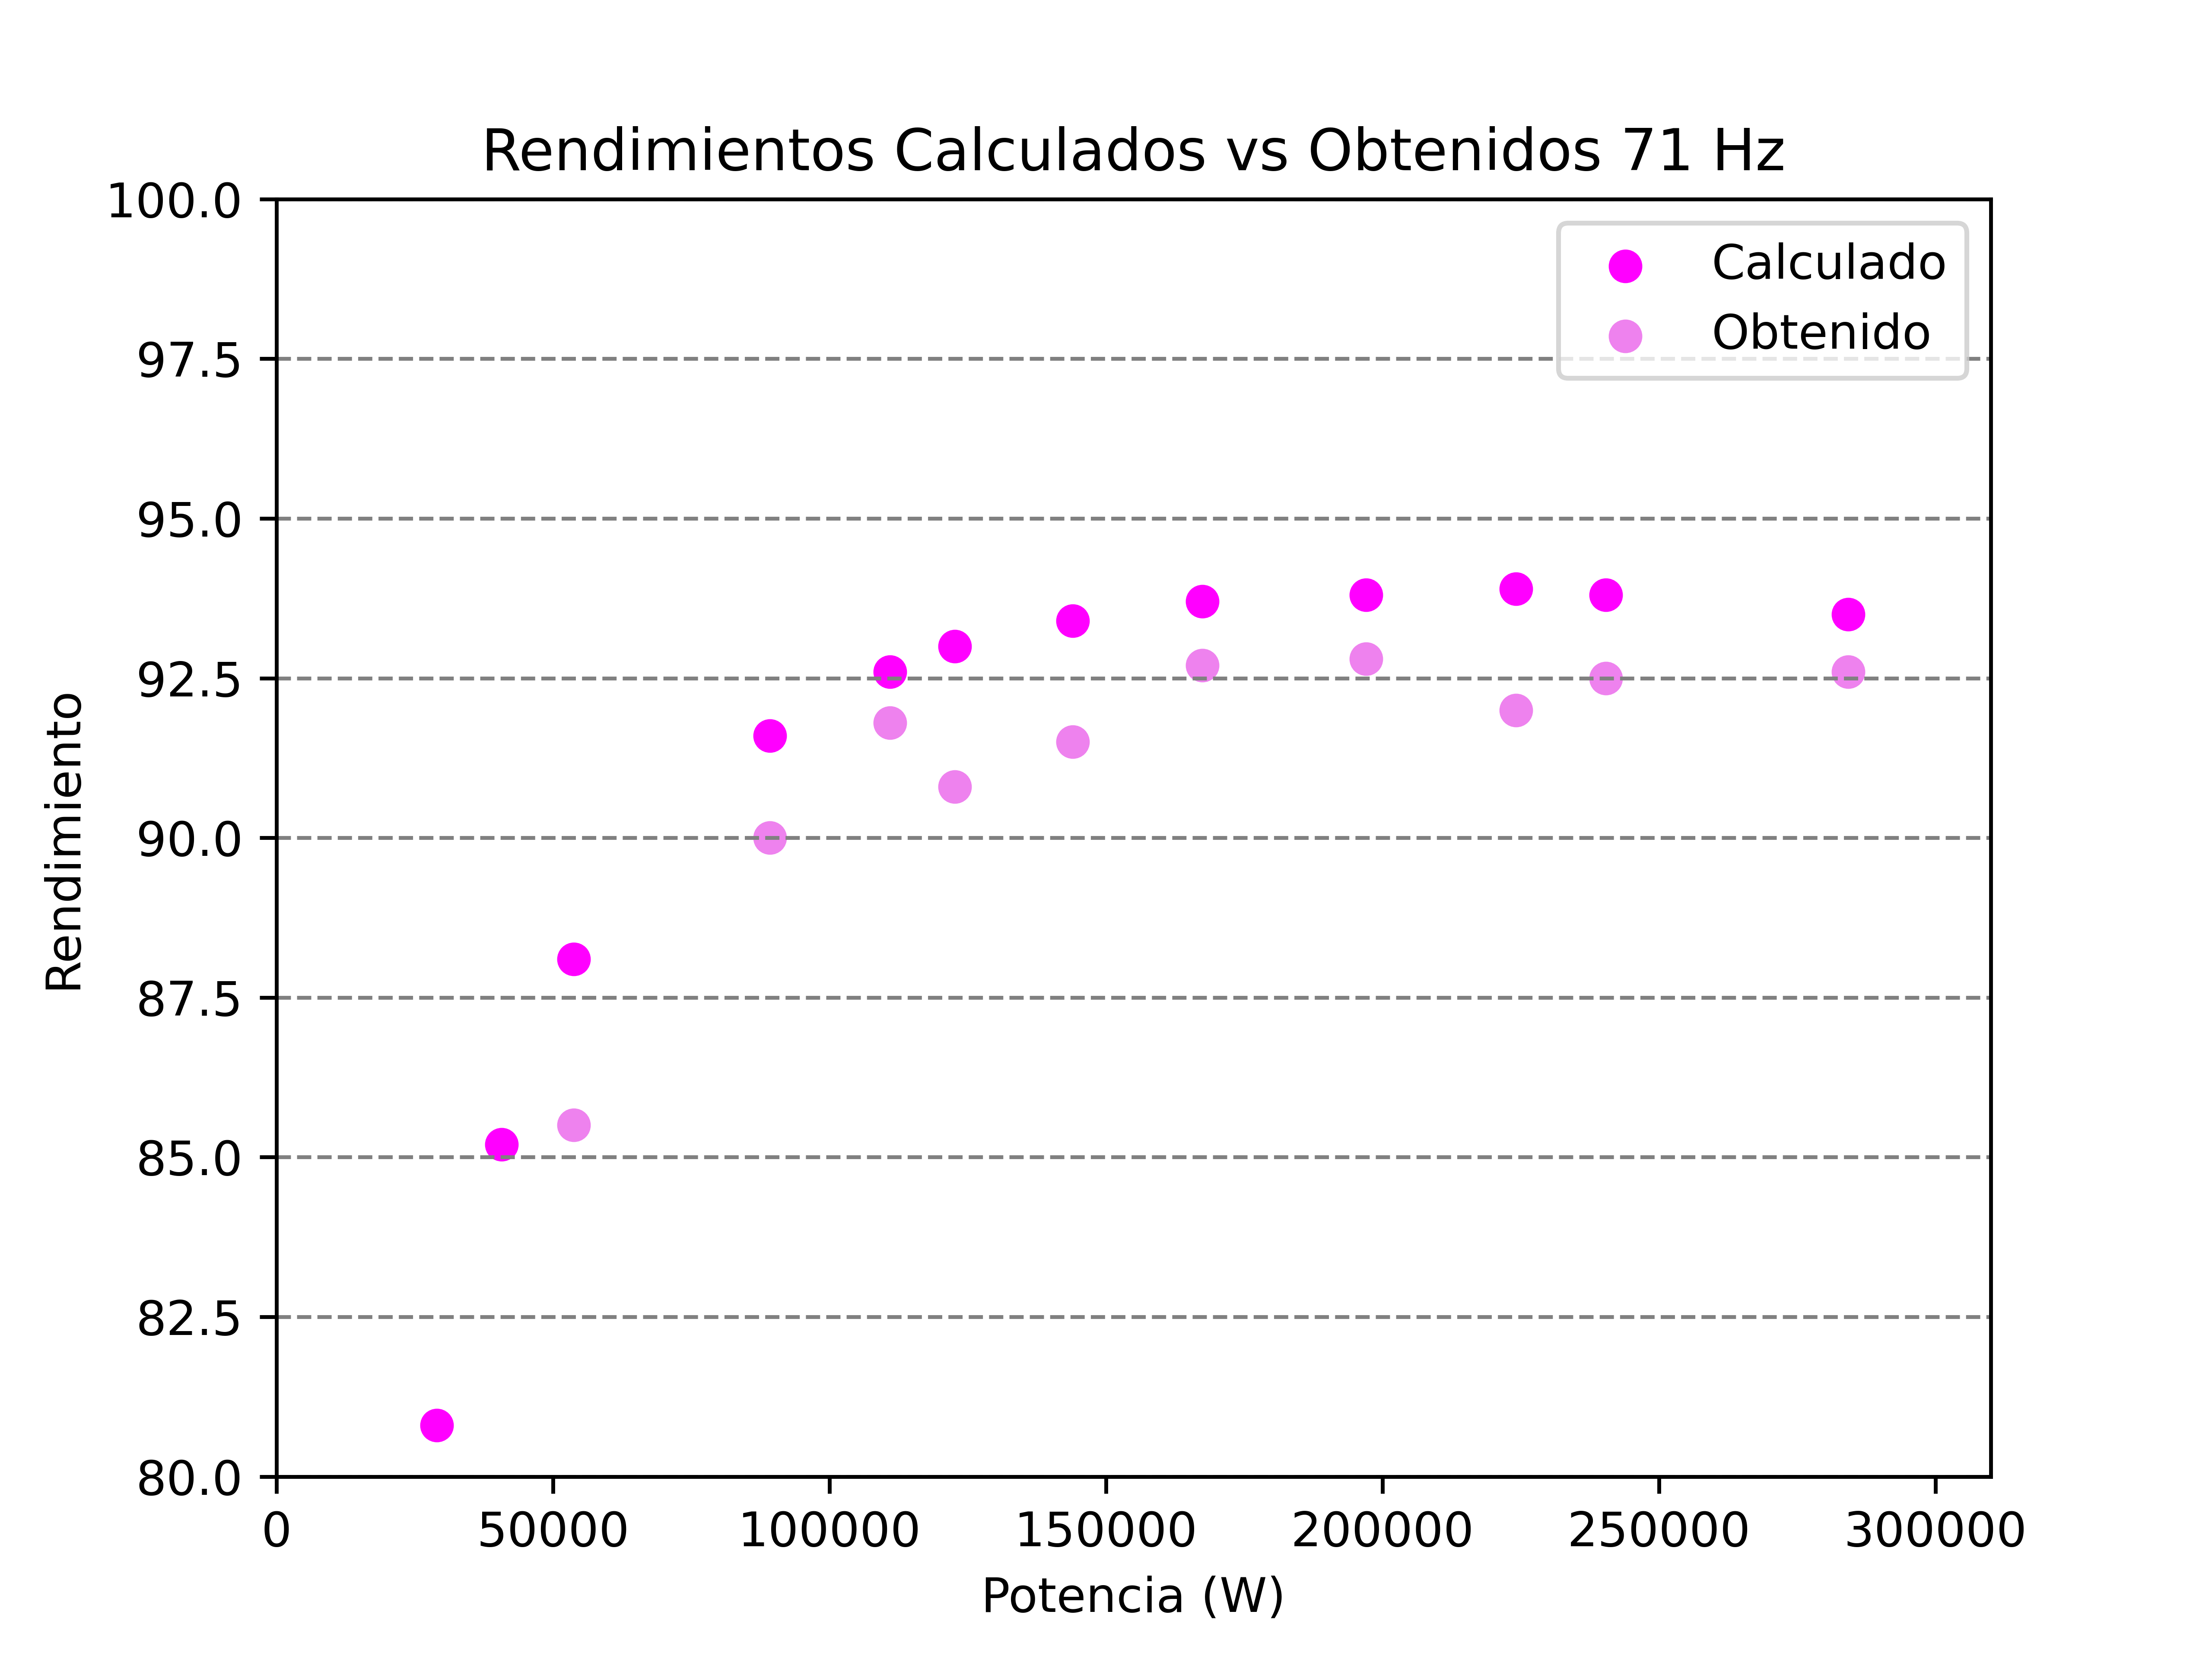
\includegraphics[ width=0.6\textwidth]{ Rendimientos Calculados vs Obtenidos 71 Hz.png }
\caption{}
\label{fig:}
\end{figure}
\begin{figure}[H]
\centering
\includegraphics[ width=0.6\textwidth]{ desviacion Rendimientos (\%) 71 Hz.png }
\caption{}
\label{fig:}
\end{figure}

\subsection{Frecuencia de 75 Hz}
\begin{figure}[H]
\centering
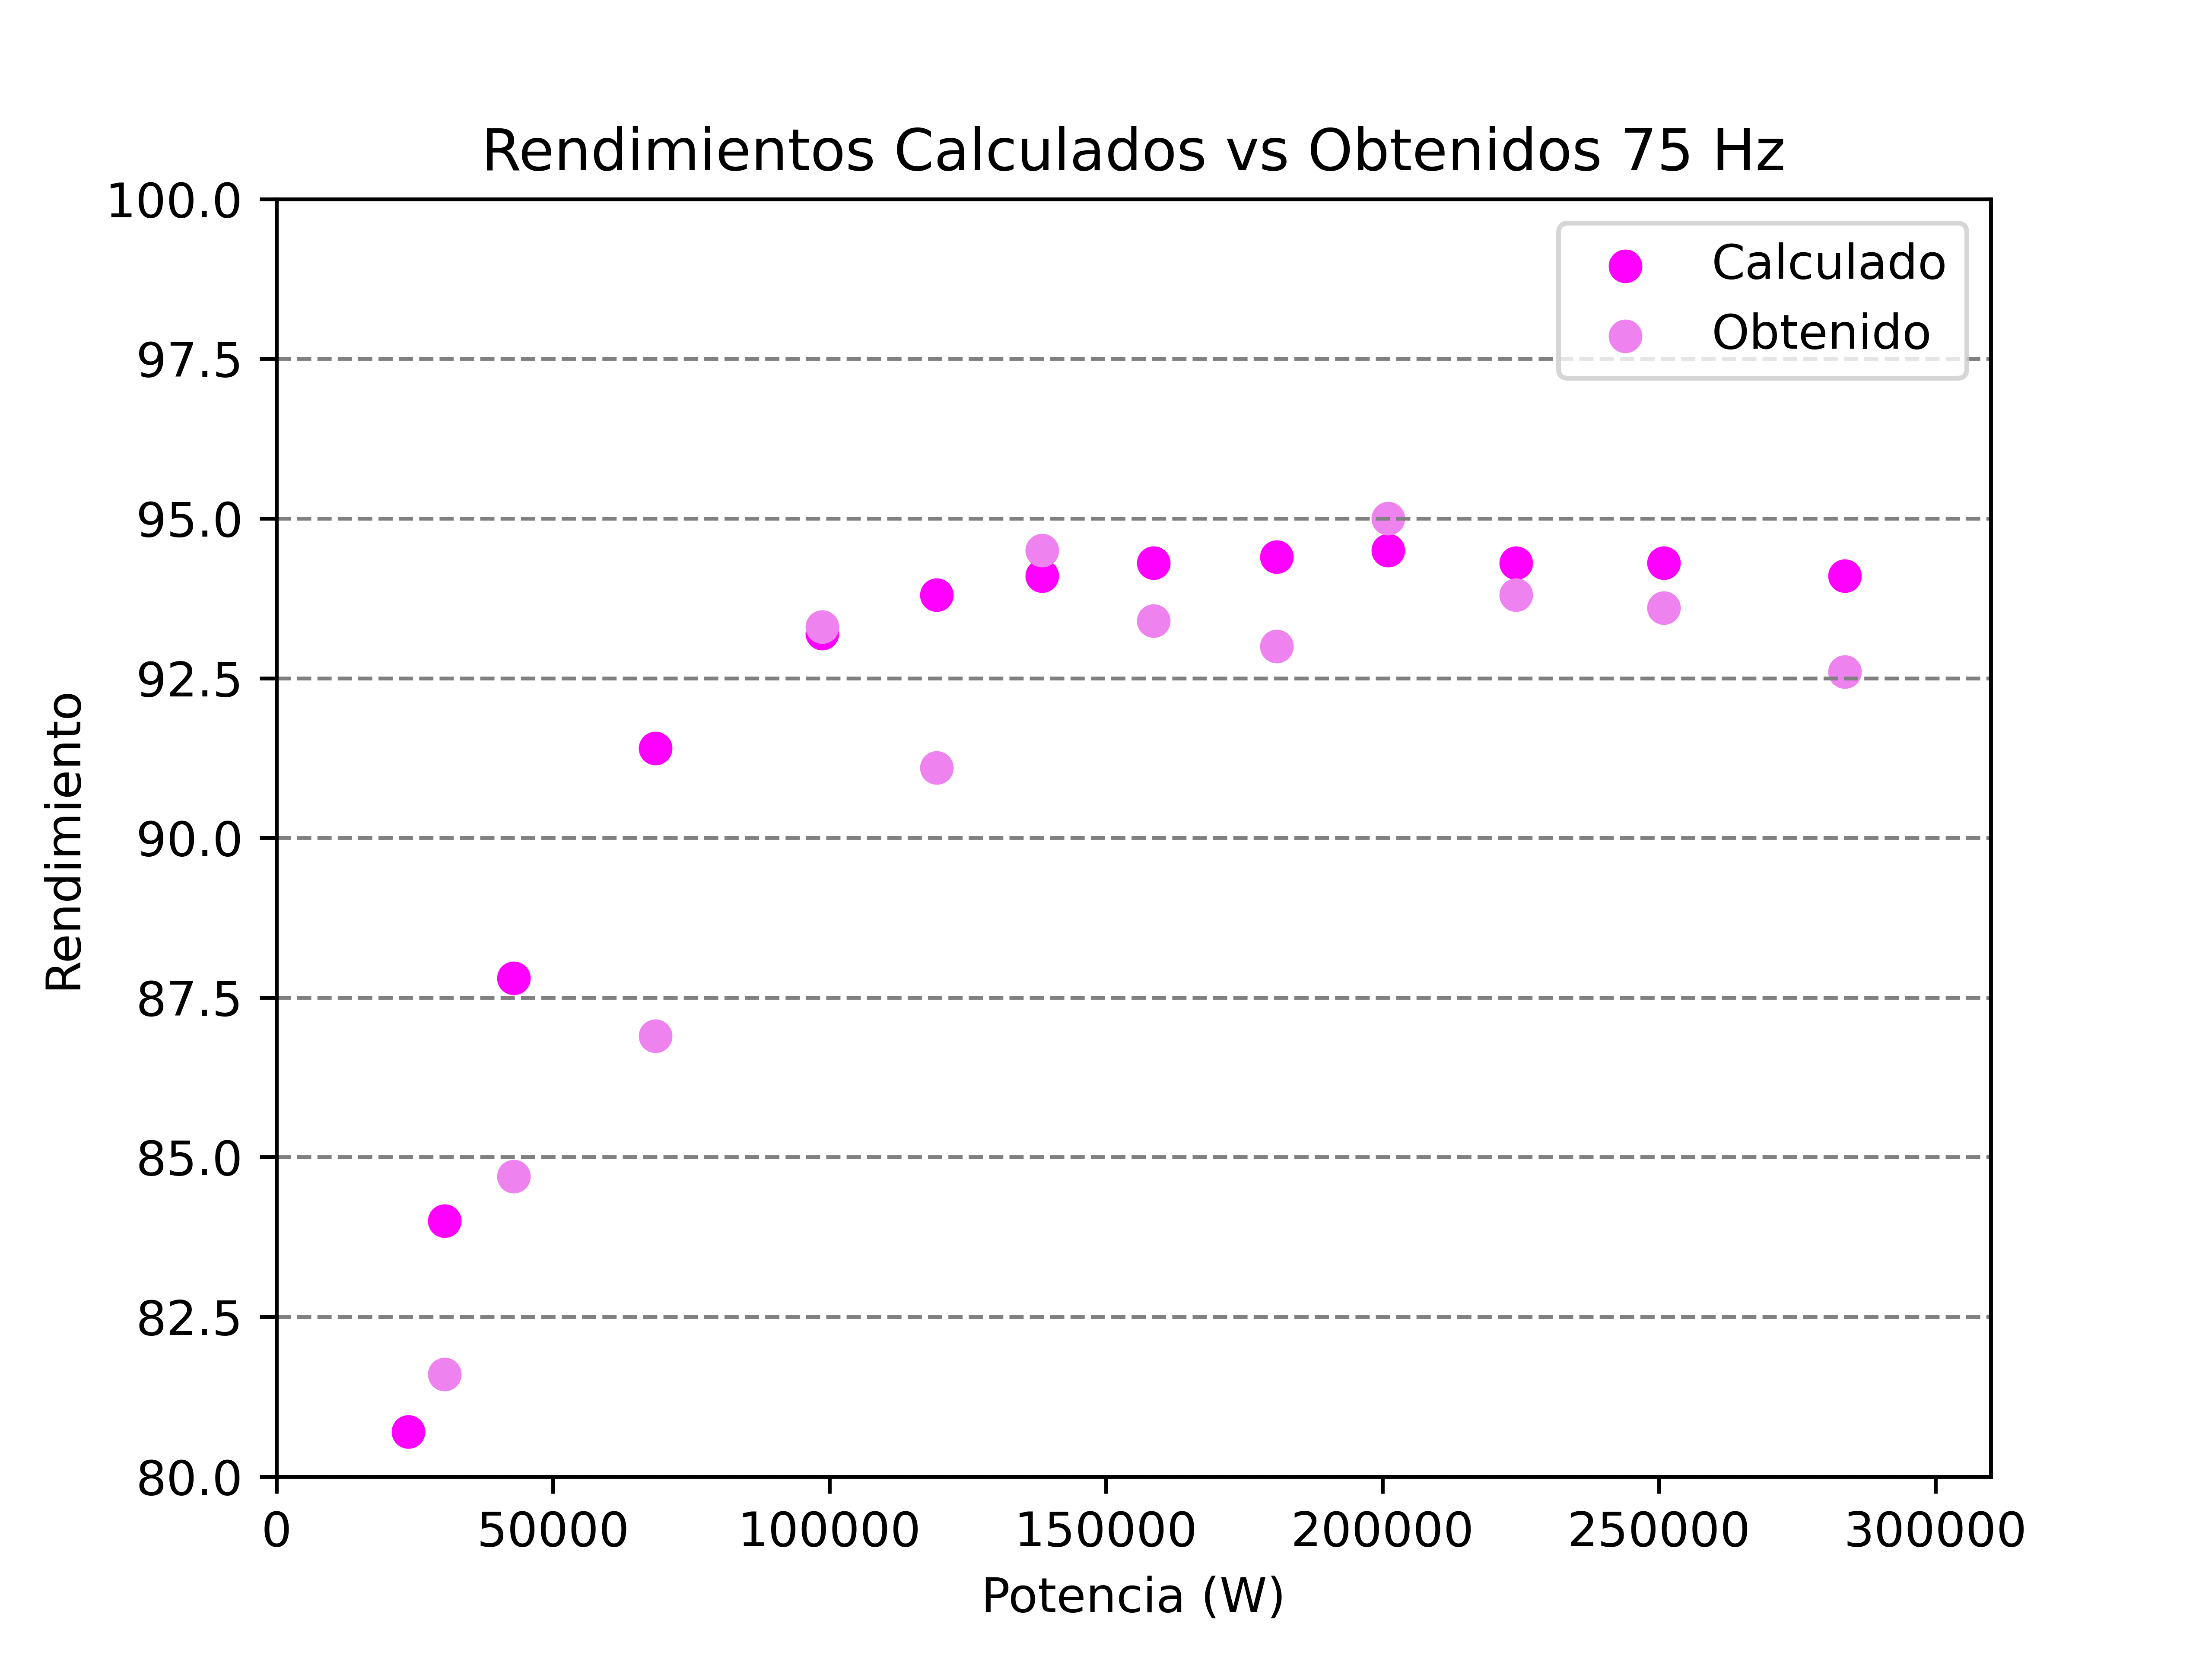
\includegraphics[ width=0.6\textwidth]{ Rendimientos Calculados vs Obtenidos 75 Hz.png }
\caption{}
\label{fig:}
\end{figure}
\begin{figure}[H]
\centering
\includegraphics[ width=0.6\textwidth]{ desviacion Rendimientos (\%) 75 Hz.png }
\caption{}
\label{fig:}
\end{figure}

\subsection{Frecuencia de 95 Hz}
\begin{figure}[H]
\centering
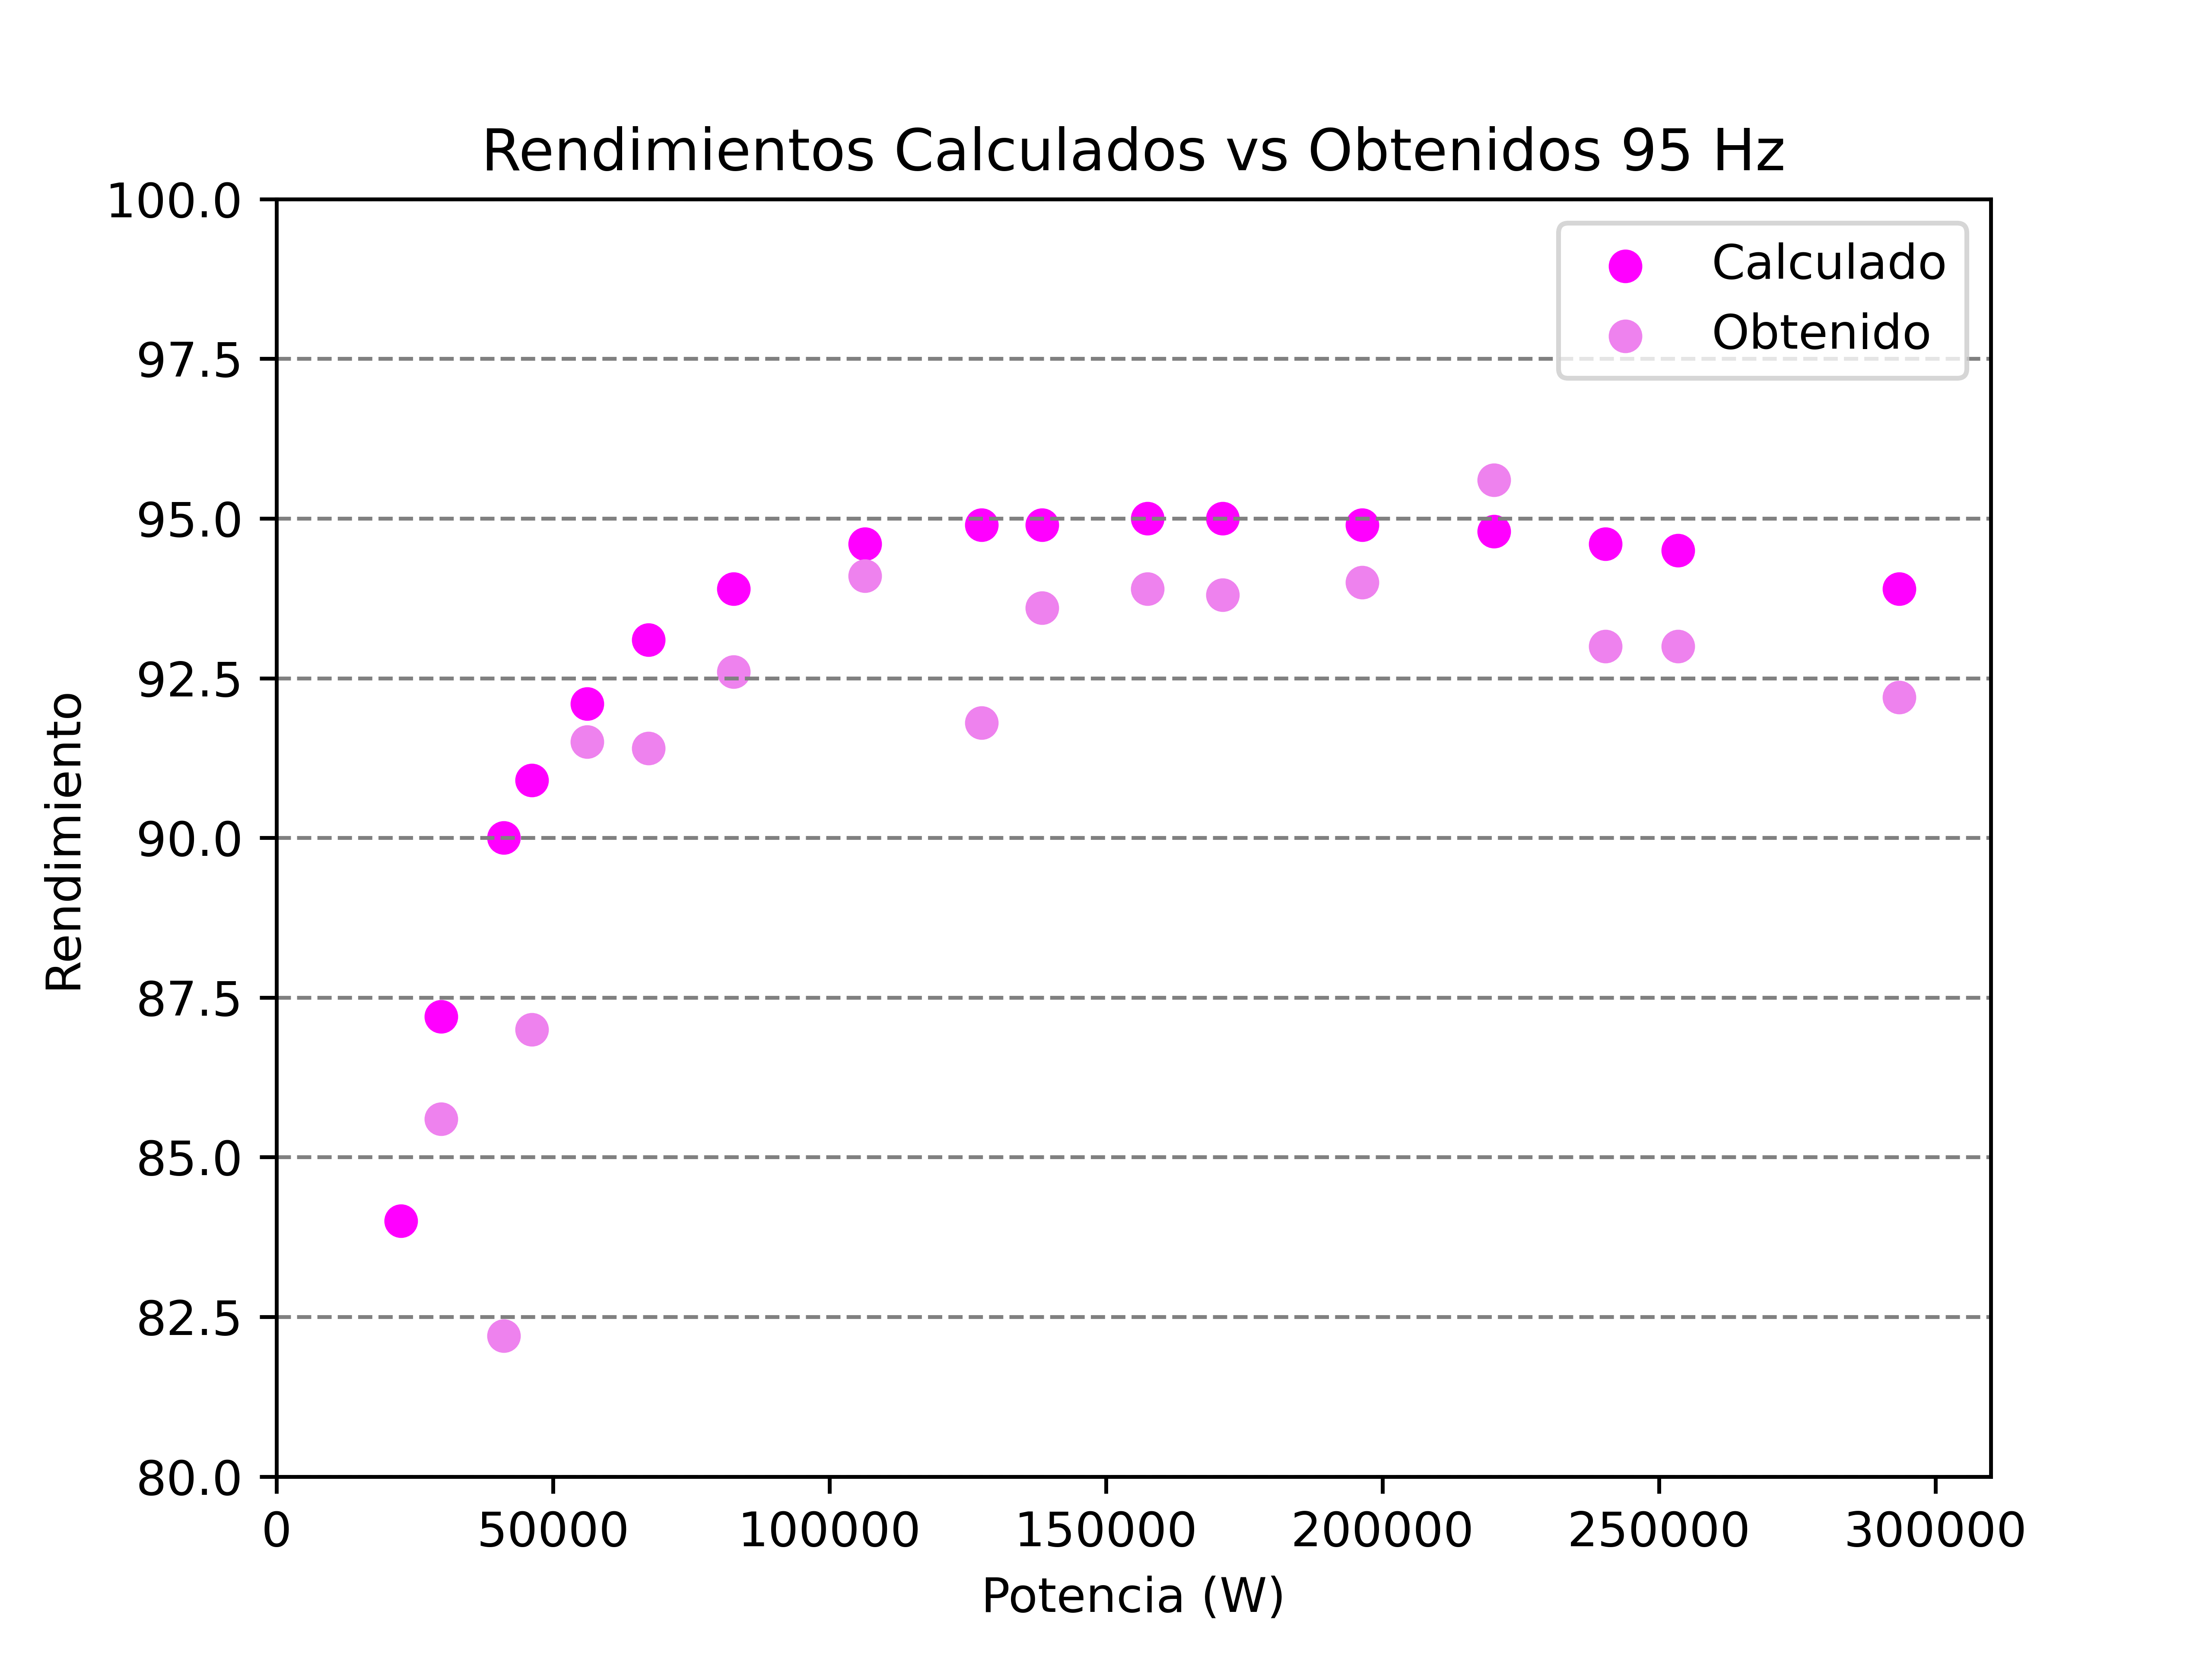
\includegraphics[ width=0.6\textwidth]{ Rendimientos Calculados vs Obtenidos 95 Hz.png }
\caption{}
\label{fig:}
\end{figure}
\begin{figure}[H]
\centering
\includegraphics[ width=0.6\textwidth]{ desviacion Rendimientos (\%) 95 Hz.png }
\caption{}
\label{fig:}
\end{figure}


\end{document}